\section{程序的机器级表示:基础知识}
\subsection{Intel处理器体系结构的历史}

\subsubsection{复杂指令集计算机(CISC)}
Intel x86系列属于复杂指令集计算机,其指令多、格式复杂。理论上 CISC 的性能较难与精简指令集计算机(RISC)相比。在低功耗场景下,其速度会受到影响。


\subsubsection{摩尔定律}
摩尔定律指出,单位面积上可以容纳的晶体管数量几乎每两年增加一倍


% \subsubsection{Intel 64位体系结构发展的历史}
% 2001年,Intel试图从IA32转变为IA64(安腾),但性能令人失望。2003年,AMD提出x86 - 64位体系结构(现称为AMD64)。2004年,Intel提出EM64T体系结构,实现对IA32的64位扩展,几乎与x86 - 64相同。2019年,英特尔宣布放弃IA64架构,目前除低端x86处理器外,其他处理器均支持x86 - 64,但仍有许多程序在32位模式下运行。
\subsection{C语言,汇编语言和机器语言}
\subsubsection{定义}
\begin{enumerate}
    \item 体系结构(指令集体系结构,ISA):编写汇编代码时需要理解的处理器设计部分,如指令集规范、寄存器组织等。
    \item 微体系结构:体系结构的具体实现,例如高速缓存大小、核心频率等。
    \item 机器语言是处理器可以直接执行的字节级程序,汇编语言是文本形式的机器语言。
\end{enumerate}
常见的指令集体系结构有Intel的x86、IA32、Itanium、x86 - 64,以及ARM(用于几乎所有移动电话)。

\subsubsection{程序员可见的状态}
\begin{enumerate}
    \item 程序计数器(PC,在x86 - 64中称为RIP),存储下一条要执行指令的地址
    \item 条件码,存储最近一次算术逻辑运算的状态信息,用于条件分支
    \item 存储器,基于字节寻址,存储程序、用户数据和栈数据
    \item 寄存器文件,频繁用于存储程序数据
\end{enumerate}

\begin{figure}[H]
    \centering
    \captionsetup{skip=4pt}
    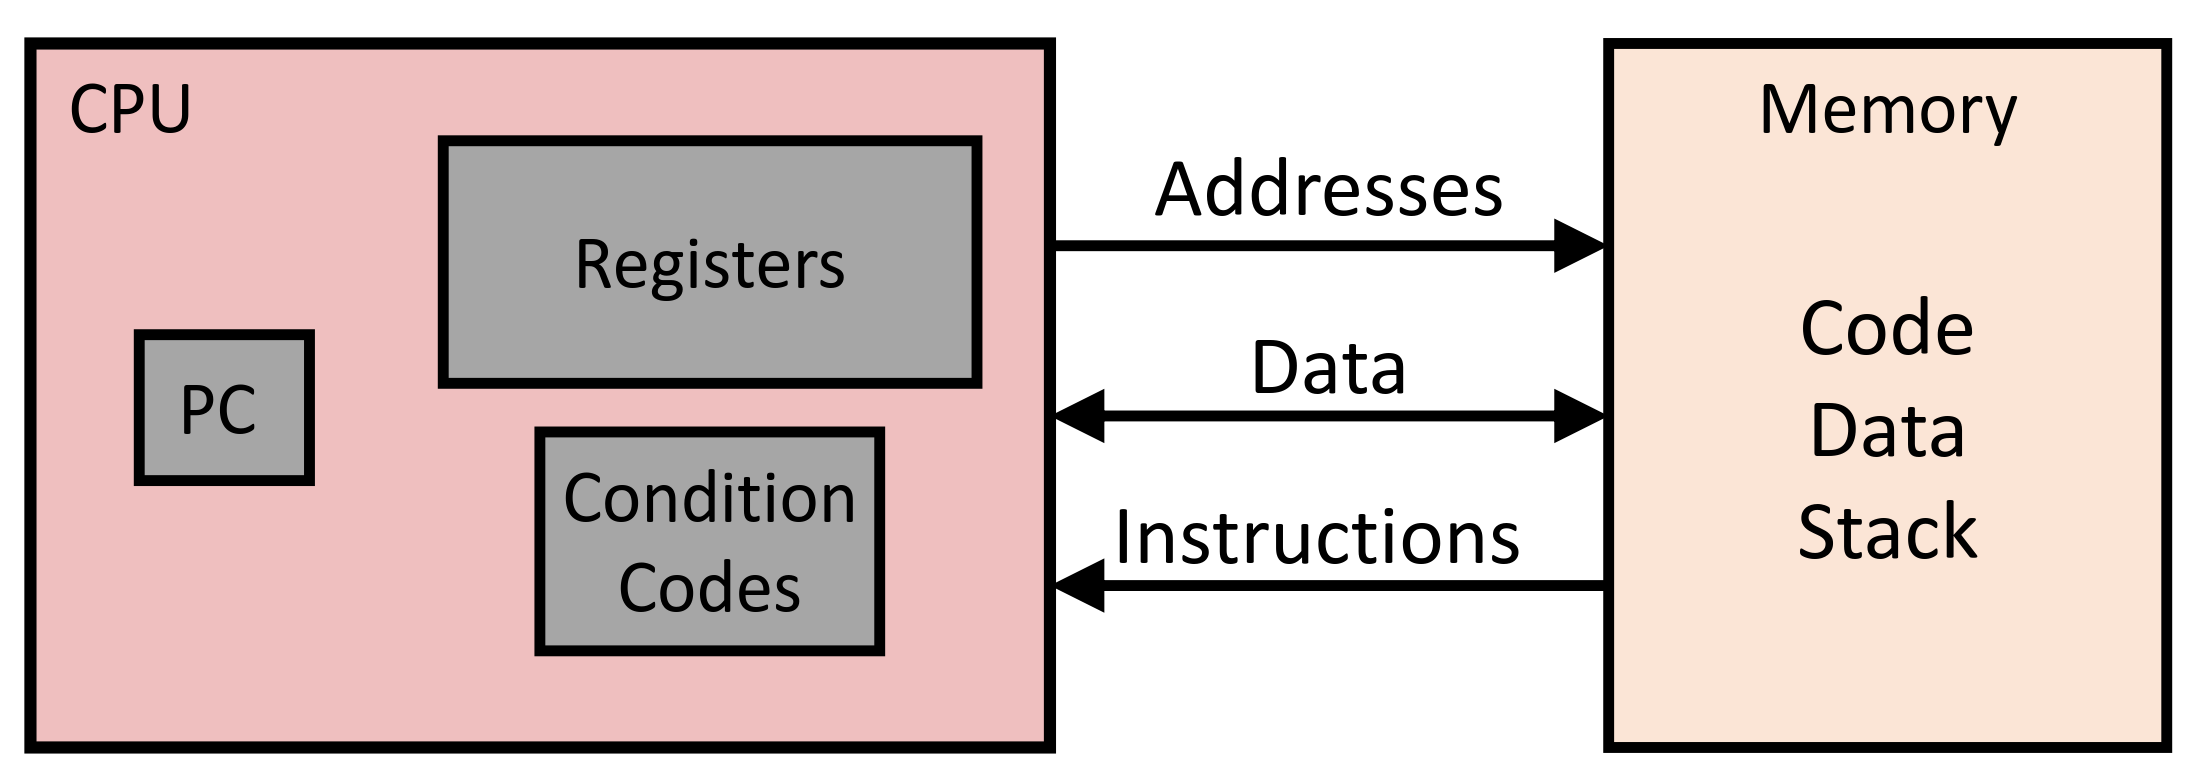
\includegraphics[width=10cm]{4.png}
    \caption{}
\end{figure}


\subsubsection{汇编语言的数据类型}
\begin{enumerate}
    \item 整数:1、2、4或8字节
    \item 地址:无类型的指针
    \item 浮点数:4、8或10字节
    \item 代码:指令的字节序列编码
\end{enumerate}
与C语言不同,汇编语言没有聚合类型,数组或结构体在汇编语言中表现为在内存中连续分配的字节。

\subsubsection{汇编语言的操作}
汇编语言可以对寄存器或存储器数据执行算术/逻辑运算,在寄存器和存储器间传输数据(包括将数据从存储器加载至寄存器以及将寄存器的数据存储至存储器),还能进行转移控制,如无条件跳转至/从过程、条件分支等。

% \subsubsection{链接器}
% 链接器将 `.s` 文件翻译为 `.o` 文件,对每条指令进行二进制编码,生成几乎完整的可执行代码,但缺少不同文件的链接信息。链接器实现了不同文件间的引用,并与静态链接库结合(例如代码中的 `malloc`、`printf` 等),某些库需要动态链接,链接在程序开始执行时进行。

\subsubsection{举例:机器指令}
对于C语言代码 \mintinline{c}{*dest = t;},对应的汇编代码 \mintinline{asm}{movq %rax, (%rbx)},将8字节数据移动至存储器。其操作数 t 存储在寄存器 \mintinline{asm}{%rax}中,dest 存储在寄存器  \mintinline{asm}{%rbx} 中,*dest 表示内存地址  \mintinline{asm}{M[%rbx]}。对应目标码(机器指令)为\mintinline{asm}{0x40059e: 48 89 03},该指令为3字节,存储于地址0x40059e。

\subsubsection{反汇编}
反汇编器是探索目标码的有用工具,它可以分析指令的编码序列,根据目标码重新生成汇编代码,并且可以对任何可执行程序文件和 \mintinline{c}{.o} 文件进行反汇编。例如使用 \mintinline{bash}{objdump –d sum} 对 sum 文件进行反汇编,或者在 gdb 调试器中使用 \mintinline{bash}{gdb sum} 以及 \mintinline{bash}{disassemble sumstore} 反汇编 sumstore 函数。反汇编程序会分析字节并重构为汇编代码。
